\section{Introducción}
\label{sec:Introduction}

En los últimos años, los multimodal large language models han logrado avances significativos en tareas de video understanding, demostrando sólidas capacidades de comprensión semántica y razonamiento en videos de distintas duraciones y escenarios \cite{li2023videochat,song2024moviechat,li2024mvbench,li2024llamavid}. Beneficiados por el pretraining a gran escala y por capacidades mejoradas de modelado cross-modal, estos modelos han sido ampliamente adoptados en diversos dominios \cite{li2024llavaov,liu2024oryx,qwen2vl,wang2025internvideo2_5}. Sin embargo, con la creciente demanda de procesamiento inteligente en tiempo real en aplicaciones online como conducción autónoma \cite{shao2024lmdrive}, live video streaming \cite{chen2025livecc} y robótica \cite{zhu2024spa}, los investigadores han desplazado cada vez más su foco desde el offline video understanding convencional hacia la tarea más desafiante de procesamiento de video en streaming~\cite{chen2024videollmonline,huang2024videochatonline,qian2024videostreaming}.


En el campo de streaming video understanding, almacenar eficientemente las características de frames de video que llegan de forma continua sigue siendo un problema desafiante y de larga data. Para mitigar la sobrecarga de almacenamiento y cómputo asociada a frames pasados, el trabajo previo ha empleado principalmente dos estrategias de reducción de características visuales: compresión durante el muestreo \cite{chen2024videollmonline,qian2024videostreaming,yao2025timechatonline} y compresión durante el almacenamiento \cite{song2024moviechat,zhang2024flashvstream,huang2024videochatonline}. La compresión durante el muestreo reduce gran parte de las características visuales entrantes, lo que limita severamente la capacidad del modelo para el razonamiento espaciotemporal fino. Como resultado, solo puede realizar una resumización semántica gruesa de la escena actual. En cambio, la compresión durante el almacenamiento suele implicar fusionar o descartar frames adyacentes según la similitud entre frames. Aunque es más eficiente en memoria, esta estrategia es propensa a perder acciones críticas en primer plano debido al ruido de fondo. También puede producir una fusión local excesiva, introduciendo irregularidades espaciotemporales que degradan la capacidad del modelo para retener y razonar sobre eventos clave a lo largo del tiempo.


\begin{figure*}[t]
        \vspace{-5pt}
	\centering
	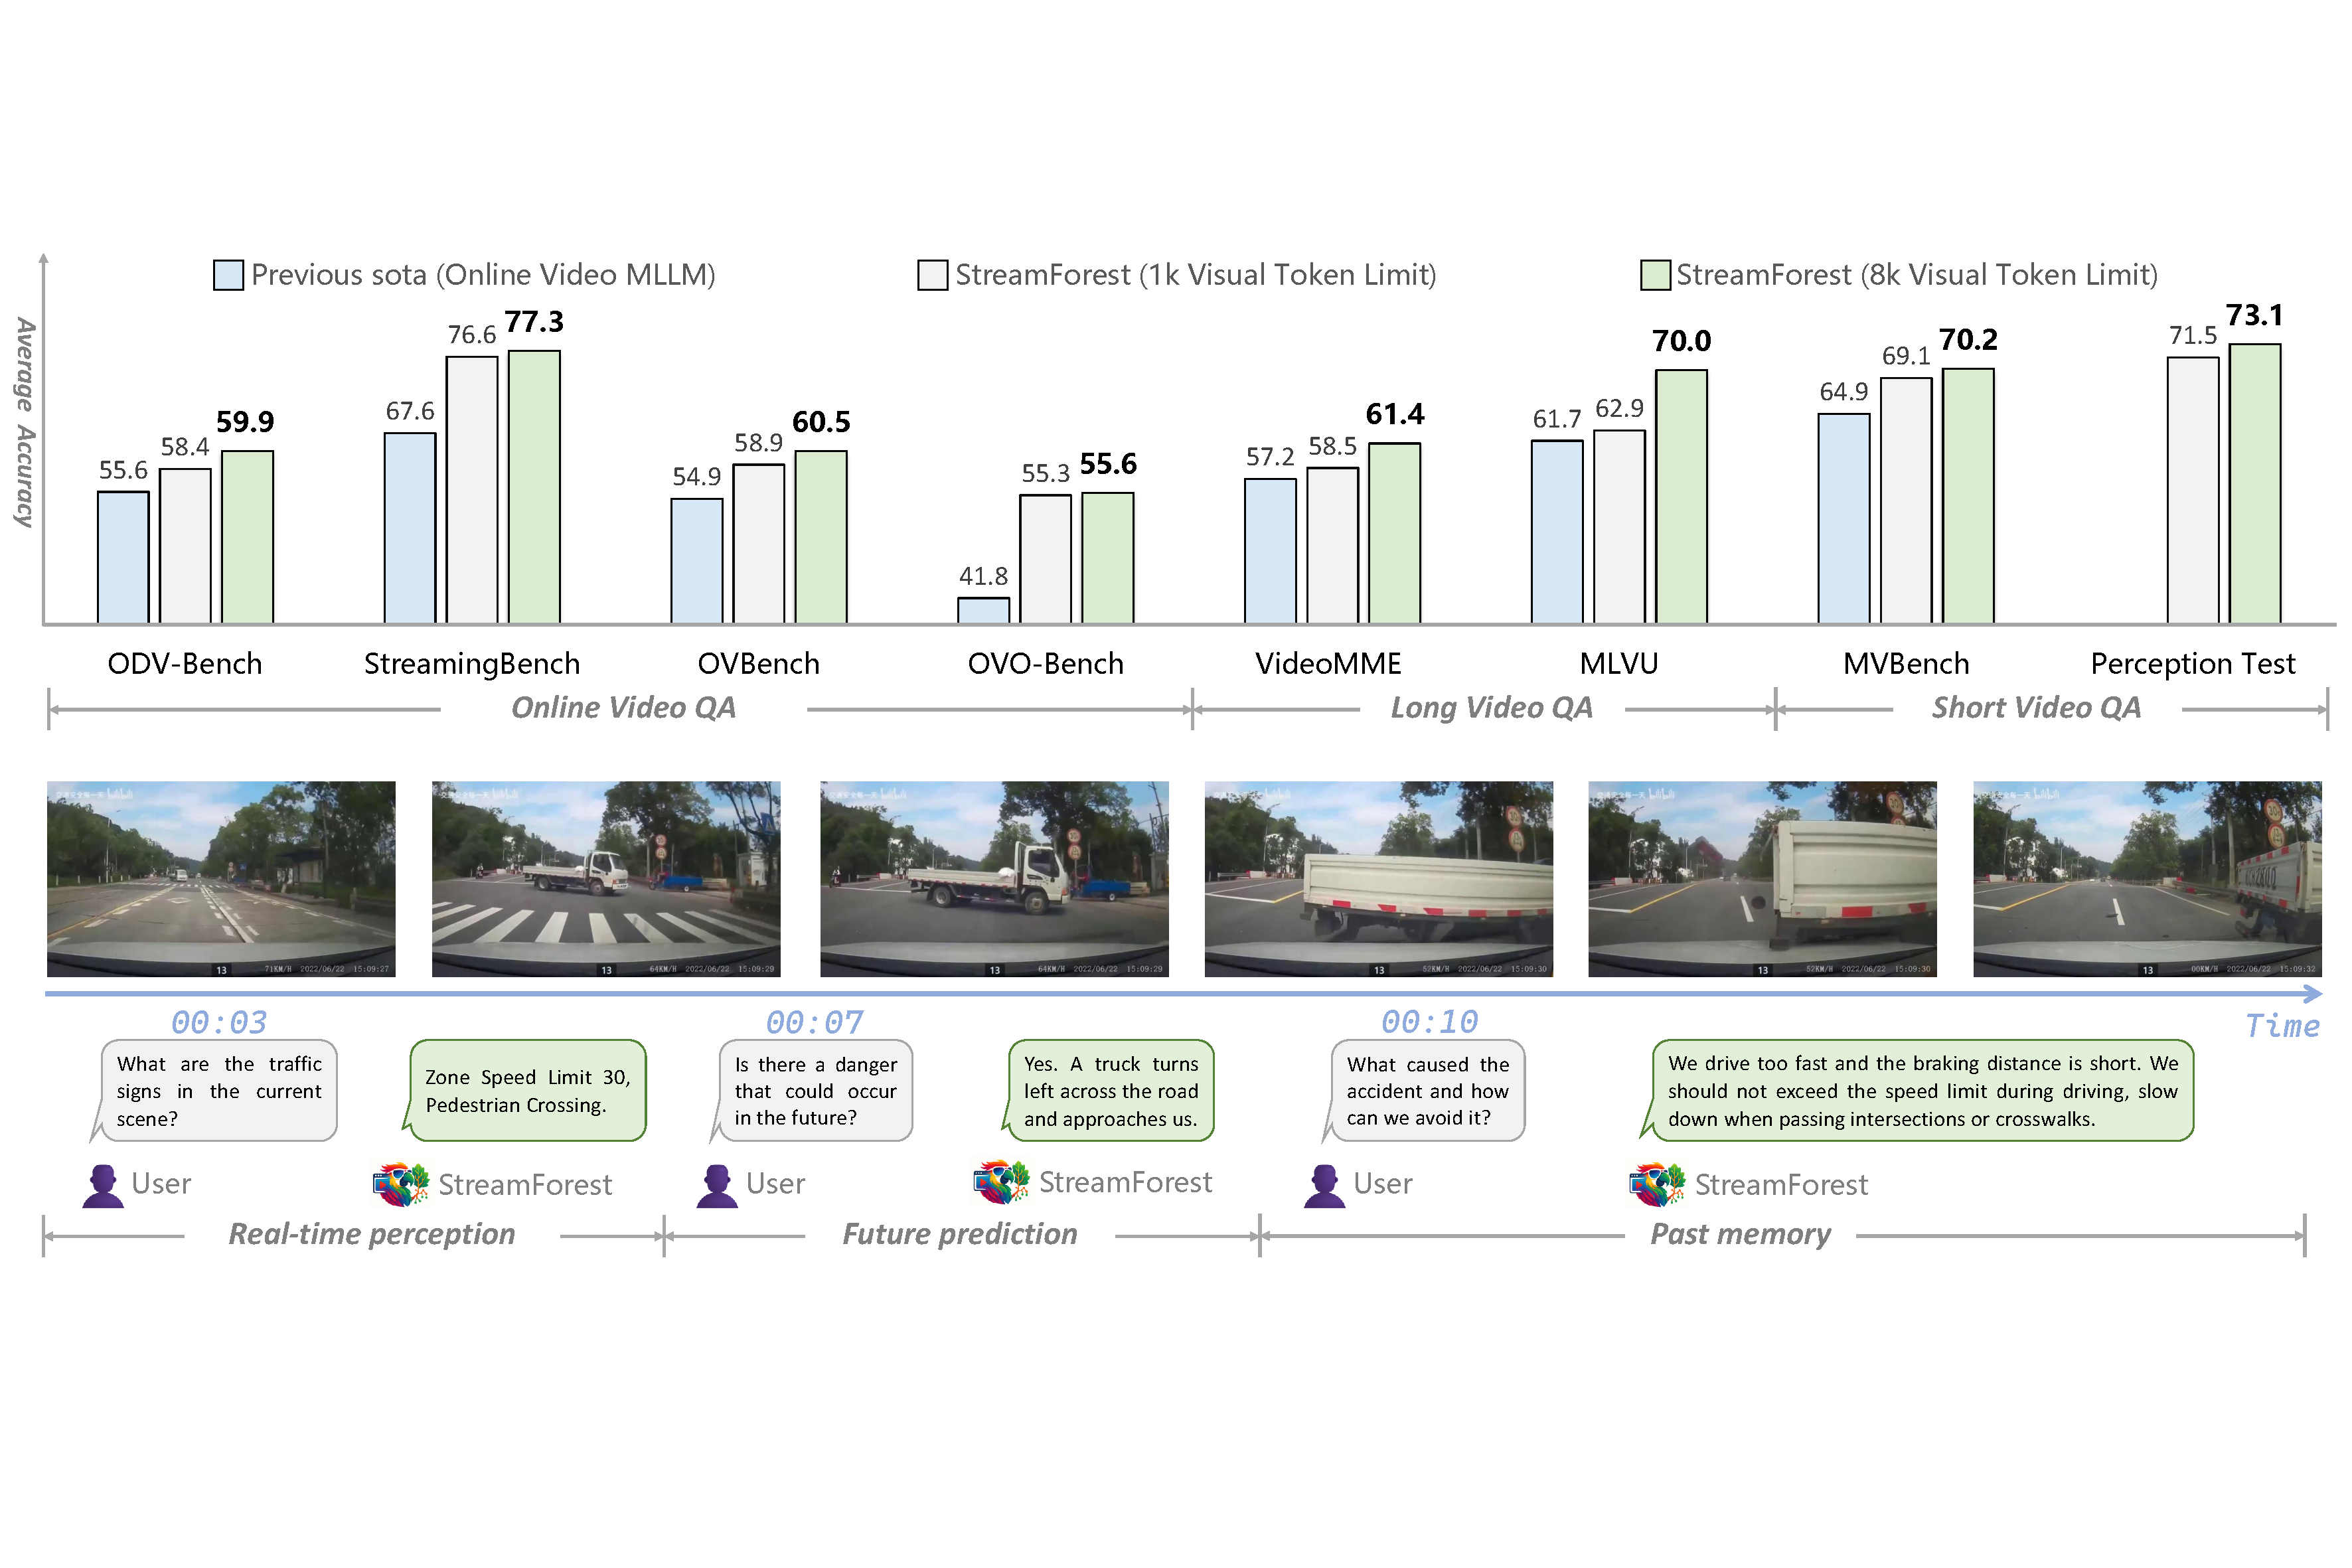
\includegraphics[width=\textwidth]{figs/introduction_img.pdf} 
	\caption{
   StreamForest logra un sólido rendimiento en diversos benchmarks de evaluación mientras utiliza significativamente menos visual tokens. Maneja eficazmente tareas clave en escenarios de streaming video, incluyendo memoria pasada, percepción en tiempo real y predicción futura.}
	\label{fig:introduction}
        \vspace{-5pt}
\end{figure*}



Para abordar los desafíos de streaming video understanding, proponemos una arquitectura novedosa llamada \textbf{StreamForest}. En su núcleo se encuentra el \textbf{Persistent Event Memory Forest}, un mecanismo diseñado para almacenar y gestionar eficientemente información visual de largo plazo. Este sistema de memoria permite que un MLLM procese streaming video ultralargo a una tasa constante de 1 fps organizando dinámicamente segmentos de video en una estructura de árbol basada en límites de eventos. La fusión de segmentos está guiada por tres funciones de penalización que consideran distancia temporal, similitud de contenido y frecuencia de fusión, garantizando una jerarquía de memoria adaptativa y significativa. Para mejorar la percepción en tiempo real, introducimos una \textbf{Fine-grained Spatiotemporal Window}, que extrae ricas características espaciotemporales locales de frames cercanos. Este módulo permite que el MLLM comprenda mejor la escena actual al enfocarse en contexto visual temporalmente relevante. También presentamos \textbf{OnlineIT}, un dataset de fine-tuning diseñado específicamente para streaming video understanding. OnlineIT mejora la capacidad del MLLM para percibir el momento presente y anticipar eventos futuros aprovechando tanto observaciones recientes como señales históricas de largo plazo. Aborda el problema de las alucinaciones causadas por cambios de distribución espaciotemporal entre frames pasados y actuales. Además, introducimos \textbf{ODV-Bench}, un nuevo benchmark para evaluar streaming video understanding en escenarios de conducción autónoma. ODV-Bench enfatiza la percepción en tiempo real y la predicción futura, proporcionando un marco sistemático para evaluar la generalización y la efectividad en el mundo real de los streaming video MLLMs en tareas downstream.

Realizamos experimentos extensivos en benchmarks tanto de online como de offline video understanding para validar la efectividad de StreamForest. Bajo la configuración por defecto con un límite de 8192 visual tokens, StreamForest supera significativamente a los MLLMs previos de estado del arte para streaming video understanding. Alcanza una exactitud promedio de 77.3\% en StreamingBench, 60.5\% en OVBench y 55.6\% en OVO-Bench. StreamForest también iguala o supera el rendimiento de los principales MLLMs de offline video understanding tanto en benchmarks de video largo como corto, a pesar de operar en una configuración de entrada de streaming video. Además, StreamForest demuestra una fuerte resiliencia bajo compresión extrema. Con un límite reducido de solo 1024 visual tokens, retiene el 96.8\% de su rendimiento promedio en ocho benchmarks en comparación con la configuración por defecto. Estos resultados resaltan la robustez y eficiencia de nuestro enfoque para procesar continuamente entradas de streaming video.
